% ============================================================
% LLM-BLM 実験 3：アナリスト予想との差を統制した決算発表のイベントの評価
% コンパイル：tectonic -X compile LLM-BLM_実験3.tex   （XeTeX 系。このフォルダで実行する）
% 図は 図/（作成スクリプト/figs.py が DB と experiments/E3_analyst_surprise/results から作る）
% 数値の出どころは experiments/E3_analyst_surprise/results/summary.json と findings.md、
% 事前登録は experiments/E3_analyst_surprise/preregistration.md
% ============================================================
\documentclass[xelatex,ja=standard,jafont=haranoaji,a4paper,10pt,openany]{bxjsreport}
\setpagelayout*{left=24mm,right=24mm,top=24mm,bottom=26mm,footskip=11mm}

\usepackage{amsmath,amssymb,mathtools,bm}
\usepackage{booktabs,array,multirow,longtable}
\usepackage{graphicx}
\usepackage{adjustbox}
\usepackage{xcolor}
\usepackage{tikz}
\usetikzlibrary{arrows.meta,positioning,calc,fit}
\usepackage{enumitem}
\usepackage{caption}
\usepackage{float}
\usepackage[most]{tcolorbox}
\usepackage[hidelinks,bookmarksnumbered]{hyperref}
\pdfstringdefDisableCommands{\def\Omega{Ω}\def\tau{τ}\def\Sigma{Σ}}

\graphicspath{{図/}}

\definecolor{c1}{HTML}{2A78D6}
\definecolor{c2}{HTML}{EB6834}
\definecolor{c3}{HTML}{1BAF7A}
\definecolor{c4}{HTML}{EDA100}
\definecolor{c7}{HTML}{6250D6}
\definecolor{ink2}{HTML}{52514E}
\definecolor{soft1}{HTML}{E4EEF9}
\definecolor{soft2}{HTML}{FBEEDF}
\definecolor{soft3}{HTML}{E3F3E9}
\definecolor{soft4}{HTML}{EEE8FA}
\definecolor{soft5}{HTML}{FDF3DA}

\newcommand{\code}[1]{\texttt{#1}}
\newcommand{\SP}{S\&P500}
\newcommand{\figref}[1]{図~\ref{#1}}
\newcommand{\tabref}[1]{表~\ref{#1}}
\newcommand{\chapref}[1]{第~\ref{#1}~章}
\newcommand{\secref}[1]{\ref{#1}~節}

\setlist[itemize]{leftmargin=1.6em,itemsep=0.2em,topsep=0.4em}
\setlist[enumerate]{leftmargin=1.8em,itemsep=0.2em,topsep=0.4em}
\captionsetup{font=small,labelfont=bf,skip=6pt}
\renewcommand{\arraystretch}{1.2}
\setlength{\LTpre}{6pt}
\setlength{\LTpost}{6pt}

\makeatletter
\def\@makechapterhead#1{\vspace*{0.3\Cvs}{\parindent\z@\raggedright\normalfont
  \ifnum\c@secnumdepth>\m@ne\if@mainmatter{\Large\headfont\@chapapp\thechapter\@chappos}\par\nobreak\vskip0.4\Cvs\fi\fi
  \interlinepenalty\@M\LARGE\headfont #1\par\nobreak\vskip 1.5\Cvs}}
\def\@makeschapterhead#1{\vspace*{0.3\Cvs}{\parindent\z@\raggedright\normalfont
  \interlinepenalty\@M\LARGE\headfont #1\par\nobreak\vskip 1.5\Cvs}}
\makeatother

\newtcolorbox{keybox}[1][要点]{enhanced,breakable,colback=soft1,colframe=c1,boxrule=0.5pt,arc=2pt,
  left=8pt,right=8pt,top=6pt,bottom=6pt,title={#1},fonttitle=\sffamily\bfseries\small,coltitle=white}
\newtcolorbox{notebox}[1][注意]{enhanced,breakable,colback=soft2,colframe=c2,boxrule=0.5pt,arc=2pt,
  left=8pt,right=8pt,top=6pt,bottom=6pt,title={#1},fonttitle=\sffamily\bfseries\small,coltitle=white}
\newtcolorbox{verdict}[1][判定]{enhanced,breakable,colback=soft4,colframe=c7,boxrule=0.5pt,arc=2pt,
  left=8pt,right=8pt,top=6pt,bottom=6pt,title={#1},fonttitle=\sffamily\bfseries\small,coltitle=white}

\tikzset{
  box/.style={draw=#1,fill=#1!8,rounded corners=2pt,align=center,font=\footnotesize,inner sep=4pt,
              minimum height=10mm,text width=24mm},
  arr/.style={-{Stealth[length=2mm]},color=ink2,line width=0.6pt},
}

\title{LLM-BLM 実験 3\\[6pt]
  \large アナリスト予想との差を統制しても、\\LLM の点数は決算発表への反応を説明するか}
\author{実験の結果の報告書}
\date{2026 年 10 月 18 日}

\begin{document}
\maketitle

% ============================================================
\chapter*{概要}
\addcontentsline{toc}{chapter}{概要}

実験 2 で、gpt-4o-mini が決算発表文から読み取った点数は、発表をはさむ 2 取引日の株価の反応を強く説明した。ただし数値の驚きは「前年同期との差（SUE）」でしか統制しておらず、LLM が本文の「予想を上回った」という記述から本当の驚きを読んでいるだけではないか、という疑問が残っていた（総合報告書 2 で最大の限界とした点）。今回は、アナリスト予想（発表前のコンセンサス EPS）と実績の差を新たに統制に加えた。手順と判定の基準は、実験 2 と同じく、計算の前に文書とコードで固定した（事前登録）。

\begin{keybox}[主な結論]
\begin{itemize}
\item \textbf{予想との差を統制しても、LLM の点数の効果はほとんど縮まない（支持）。}1 標準偏差あたり $+120$bp が $+116$bp になっただけで、97\% が残った（$t$ 9.37、置換の対照で $p=0.001$）。
\item \textbf{予想との差そのものも効く}（$+69$bp、$t$ 6.2）。データは確かに働いている。それでも LLM の効果は、予想との差の約 1.7 倍だった。
\item \textbf{LLM は予想との差を少しは読んでいるが、主な情報は別にある。}予想を上回った発表の中でも、下回った発表の中でも、LLM の点数が高いほど反応が良い。
\item \textbf{取引に使える価値は、やはりない。}発表の後 2〜21 日のドリフトは有意でない（$+9$bp、$t$ 0.8）。
\end{itemize}
\end{keybox}

\textbf{意味}：LLM の読み取りは、EPS の予想との差という「数字の驚き」には還元できない。ガイダンスや見通しの書き方など、文章の中身を読んでいると考えられる。ただし、売上の予想とガイダンスの予想はまだ統制していない。

\setcounter{tocdepth}{1}
{\small\tableofcontents}

% ============================================================
\chapter{目的}\label{ch:intro}

実験 2 の主な結果は次のとおりだった。

\begin{itemize}
\item gpt-4o-mini の合成点数（語調＋見通し＋ガイダンスの変更）が 1 標準偏差高いと、発表をはさむ 2 取引日の超過リターンは $+120$bp 高い（$t$ 9.41）。
\item 辞書・FinBERT・TF-IDF・SUE を統制しても変わらず、効果は FinBERT や TF-IDF の約 3 倍。
\item 発表の後のドリフトは有意でない。
\end{itemize}

残っていた疑問は、「LLM は、本文の『予想を上回った』『市場予想を下回る見通し』といった記述から、アナリスト予想との差（本当の驚き）を読んでいるだけではないか」である。SUE は前年同期との差なので、市場が何を期待していたかは表さない。もしこの疑問のとおりなら、予想との差を統制すると、LLM の効果は大きく縮むはずである。

\begin{verdict}[問い]
アナリスト予想との差を統制しても、gpt-4o-mini の合成点数は、発表への株価の反応を説明するか。
\end{verdict}

% ============================================================
\chapter{データ}\label{ch:data}

\section{アナリスト予想}

Alpha Vantage の EARNINGS から、各四半期の発表前のコンセンサス EPS と実績 EPS、発表日、発表の時間帯（寄り前・引け後）を取得した（2016 年以降に決算発表がある 656 銘柄）。

\begin{itemize}
\item 1 銘柄 1 回の問い合わせで、過去の全四半期が返る（多くの銘柄で 1996 年から）。無料の枠（1 日 25 回）で取得した。
\item 予想がなかった 77 銘柄のうち 73 銘柄は、買収や上場廃止で今はない会社で、株価がないため評価の標本には入っていない。残りの 4 銘柄（BRK-B、BF-B、BXP、DOC）は種類株や REIT である。
\item 利用規約は個人の非商用の研究を認めているが、再許諾できない。予想の値そのものは Git に入れず、DB とキャッシュにだけ置いた。
\end{itemize}

\section{決算発表との照合}

発表の受理日（ニューヨーク時間）に最も近い報告日を持つ同じ銘柄の四半期を、前後 3 日以内で選んだ。全期間の 23,765 本では 95.0\% が照合でき、そのうち 91\% は同じ日だった。

\begin{table}[H]
\centering
\caption{実験 2 の時間帯の区分と、データ上の発表の時間帯（全期間）。}
\small
\begin{tabular}{lrr}
\toprule
実験 2 の時間帯（受理時刻） & データ上の寄り前 & データ上の引け後 \\
\midrule
場中（9:30〜16:00） & 7,054 & 281 \\
17:30 以後 & 540 & 5,275 \\
引け後（16:00〜17:30） & 188 & 4,160 \\
寄り前（〜9:30） & 4,964 & 106 \\
\bottomrule
\end{tabular}
\end{table}

「場中に受理された 8-K の多くは、寄り前に配信された発表」という実験 2 の推測が確かめられた。反応の日の決め方が誤るのは、場中に受理されたがデータ上は引け後の発表（281 本、約 1.2\%）で、反応の日が 1 日早くなる。主な窓（2 取引日）はその翌日も含むので、影響は小さい。

\section{標本}

実験 2 の標本 A（2023 年 11 月〜2026 年 8 月、5,374 本、527 の発表日）をそのまま使った。そのうち 5,200 本（96.8\%）に予想があった。予想を上回った発表が 4,086 本、一致が 229 本、下回りが 894 本である。\textbf{標本 A は、実験 2 で発表への反応を一度計算した期間の再利用である。}

% ============================================================
\chapter{方法と事前登録}\label{ch:method}

事前登録の文書（\code{experiments/E3\_analyst\_surprise/preregistration.md}）と評価のコード（\code{run.py}）を、コミット \code{1f39810} に固定してから、1 回だけ実行した。評価のコードは、作ったデータで次の 2 つを見分けられることを確かめてある。
\begin{itemize}
\item LLM の点数が予想との差とは別の情報を持つ場合 → 統制の後も係数が残る。
\item LLM の点数が予想との差をなぞっているだけの場合 → 統制で係数が消える。
\end{itemize}

\begin{table}[H]
\centering
\caption{主な検定の設計。}
\small
\begin{tabular}{lp{10.6cm}}
\toprule
モデル M0 & 実験 2 の主な検定と同じ（目的変数、LLM の合成点数、統制、固定効果、丸め、標準化） \\
モデル M1（主） & M0 に、予想との差（（実績 $-$ 予想）$\div$ |予想|、上下 1\% で丸めて標準化）と、照合できなかった印を加える \\
判定 & M1 の LLM の係数が、t 検定（発表日ごとにまとめた標準誤差）と、同じ発表日の中での置換 1,000 回の両方で片側 $p<0.05$ なら「支持」 \\
副次（Holm） & S1 予想との差の係数、S2 発表の後のドリフト、S3 LLM の点数は予想との差を読んでいるか \\
頑健性 & R1 上回り・下回りの印、R2 順位の版、R3 照合と時刻のずれを除く、R4 驚きを丸めない \\
\bottomrule
\end{tabular}
\end{table}

% ============================================================
\chapter{結果}\label{ch:result}

\section{主な検定}

\begin{verdict}
\textbf{支持。}M1 の LLM の合成点数の係数は、1 標準偏差あたり $+116$bp（95\% 区間 $+92$〜$+141$bp、$t=9.37$）。置換の対照の片側 $p=0.001$。M0（$+120$bp）に対して 97\% が残った。
\end{verdict}

\begin{figure}[H]
\centering
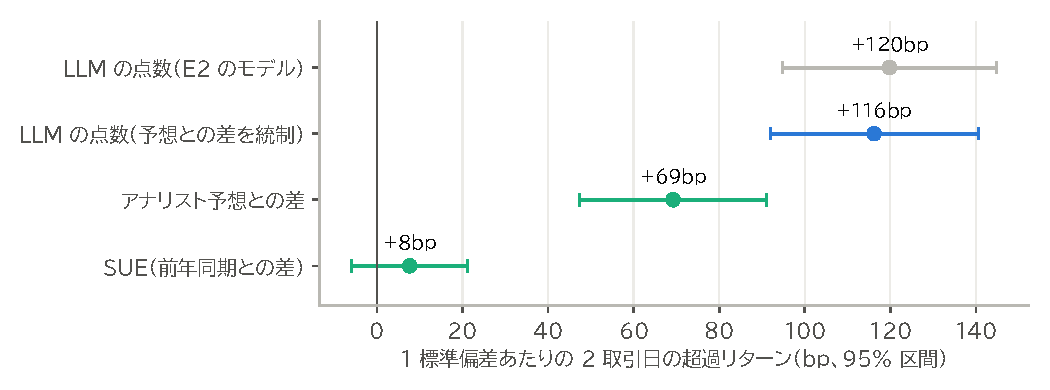
\includegraphics[width=0.92\linewidth]{coefficients.pdf}
\caption{LLM の点数の係数（予想との差を統制する前と後）と、主なモデルでの数値の驚きの係数（1 標準偏差あたり、95\% 区間）。}
\label{fig:coef}
\end{figure}

予想との差そのものは $+69$bp（$t$ 6.2）で、反応を確かに説明する（\figref{fig:coef}）。一方、前年同期との差（SUE）は、予想との差を入れると $+8$bp（$t$ 1.1）に縮んだ。市場が反応するのは「前年との差」ではなく「予想との差」であり、データはその点で筋が通っている。

\section{予想を上回った発表と、下回った発表の中で}

\begin{figure}[H]
\centering
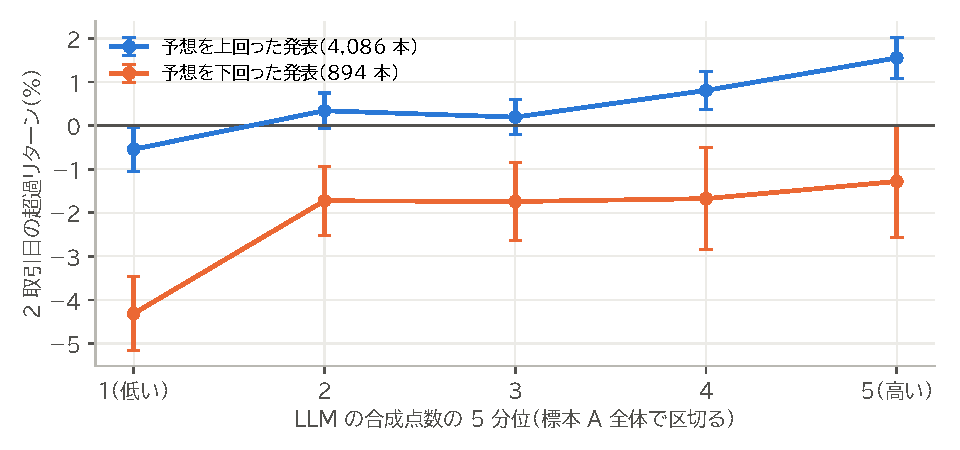
\includegraphics[width=0.85\linewidth]{within_groups.pdf}
\caption{LLM の合成点数の 5 分位ごとの、2 取引日の超過リターンの平均（予想を上回った発表と、下回った発表に分けて。上下 1\% で丸め、縦線は 95\% 区間）。探索の図で、判定には使っていない。}
\label{fig:within}
\end{figure}

\begin{table}[H]
\centering
\caption{LLM の合成点数の 5 分位ごとの、2 取引日の超過リターンの平均（\%、探索）。}
\small
\begin{tabular}{lrrrrr}
\toprule
& 1（低い） & 2 & 3 & 4 & 5（高い） \\
\midrule
予想を上回った発表（4,086 本） & $-0.54$ & $+0.34$ & $+0.20$ & $+0.81$ & $+1.56$ \\
予想を下回った発表（894 本） & $-4.31$ & $-1.72$ & $-1.74$ & $-1.68$ & $-1.28$ \\
\bottomrule
\end{tabular}
\end{table}

予想を上回った発表の中でも、点数が高いほど反応が良く、最も低い 5 分位では上回ったのに平均で下げている（\figref{fig:within}）。予想を下回った発表では、点数が最も低い 5 分位だけが大きく下げた（$-4.31\%$）。EPS は予想を下回り、しかも文章の中身（ガイダンスの引き下げ、見通しの悪化など）も悪い発表である。

\section{副次の分析と頑健性}

\begin{table}[H]
\centering
\caption{副次の分析（Holm で 3 つを補正）。}
\small
\begin{tabular}{lrrr}
\toprule
& 係数 & $t$ & Holm の $p$ \\
\midrule
S1 予想との差の係数（M1） & $+69$bp & 6.20 & $<0.001$ \\
S2 発表の後のドリフト（2〜21 日目） & $+9$bp & 0.77 & 0.22 \\
S3 LLM の点数 → 予想との差 & $+1.4$ ポイント & 2.90 & 0.004 \\
\bottomrule
\end{tabular}
\end{table}

\begin{figure}[H]
\centering
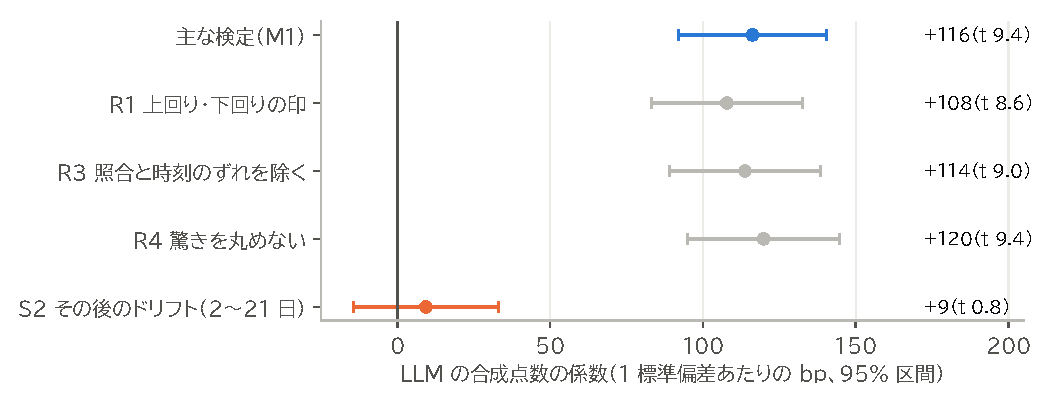
\includegraphics[width=0.92\linewidth]{robustness.pdf}
\caption{LLM の合成点数の係数の頑健性。R2（順位の版）は単位が違うので省いた（$t$ 6.43）。}
\label{fig:robust}
\end{figure}

\begin{itemize}
\item \textbf{S3}：LLM の点数が 1 標準偏差高い発表は、予想との差が平均 1.4 ポイント大きかった。LLM は予想との差を少しは読んでいるが、その部分は効果のごく一部である。
\item \textbf{頑健性}：上回り・下回りの印にしても（R1、上回りの印は $+266$bp）、順位にしても（R2）、照合できなかった発表と時刻のずれを除いても（R3）、驚きを丸めなくても（R4）、LLM の係数は $+108$〜$+120$bp、$t$ は 6.4〜9.4 だった（\figref{fig:robust}）。R4 では、驚きの裾が長すぎて予想との差の係数が消えるが、LLM の係数は変わらない。
\end{itemize}

% ============================================================
\chapter{考察と限界}\label{ch:discussion}

\section{LLM は何を読んでいるか}

実験 2 の後に残っていた「LLM は本当の驚き（EPS の予想との差）を文章から読んでいるだけ」という説明は、データで否定された。予想との差を統制しても係数は 97\% 残り、予想を上回った発表の中でも下回った発表の中でも、点数は反応を説明した。LLM が読んでいるのは、EPS の数字の驚き以外の中身（ガイダンスの変更、需要や受注の見通し、経営陣の語調）と考えられる。実験 2 の項目ごとの分析で、語調・見通し・ガイダンスがどれも単独で効いたこととも合う。

\section{取引と BLM にとっての意味}

予想との差を統制しても、発表の後のドリフトは有意でなかった。LLM の読み取りが正確でも、その中身は 2 日のうちに株価に入る。BLM のビューにする価値がないという実験 2 の結論は変わらない。

\section{限界}

\begin{itemize}
\item \textbf{売上の予想とガイダンスの予想は統制していない。}無料で取れる予想は EPS だけだった。LLM の効果の一部は、売上の驚きや、会社の見通しと市場の期待の差を、文章から読んでいる可能性が残る。
\item \textbf{予想との差の測り方}：$\div$ |予想| で測ったので、予想が 0 に近い発表で値が極端になる。丸めと順位の版で確かめた。株価で割る測り方は、EPS と株価の株式分割の扱いが揃わないので使わなかった。
\item \textbf{予想のデータの元}（どの会社の集計か）は公開されていない。
\item \textbf{標本 A は、実験 2 で一度見た期間}である。新しい統制を加えた検定として事前登録したが、確認の強さは、結果を見ていない標本での検定より一段弱い。
\end{itemize}

% ============================================================
\chapter*{再現の手順}
\addcontentsline{toc}{chapter}{再現の手順}

\begin{verbatim}
python run_events.py estimates                 # 予想（無料の枠は 1 日 25 銘柄）
python experiments/E2_event_reaction/run.py    # 実験 2 の panel.csv
python experiments/E3_analyst_surprise/run.py  # 事前登録の後に 1 回
cd 資料集/02_実験/実験3_アナリスト予想
python 作成スクリプト/figs.py                   # この資料の図
\end{verbatim}

数値の出どころは \code{experiments/E3\_analyst\_surprise/results/summary.json} と \code{findings.md}。費用は 0 円（予想は無料の枠、計算はこの PC）。

\end{document}
